\begin{figure}[H]
    \centering
    \definecolor{pressureblue}{RGB}{30,95,175}
    \definecolor{resultred}{RGB}{190,45,45}
    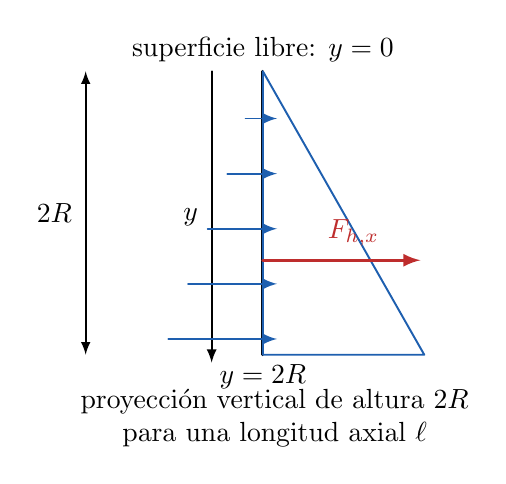
\begin{tikzpicture}[x=1cm,y=1cm,line cap=round,line join=round]
        % Proyección vertical de la superficie curva
        \draw[line width=1.0pt] (4.00,0.55) -- (4.00,4.15);
        \node[above] at (4.00,4.15) {superficie libre: $y=0$};
        \node[below] at (4.00,0.55) {$y=2R$};

        % Eje de profundidad
        \draw[-latex,line width=0.65pt] (3.35,4.15) -- (3.35,0.45);
        \node[left] at (3.30,2.30) {$y$};

        % Cota 2R
        \draw[latex-latex,line width=0.6pt] (1.75,0.55) -- (1.75,4.15);
        \node[left] at (1.70,2.35) {$2R$};

        % Presiones elementales crecientes hacia el fondo
        \draw[pressureblue,-latex,line width=0.70pt] (3.78,3.55) -- (4.18,3.55);
        \draw[pressureblue,-latex,line width=0.70pt] (3.55,2.85) -- (4.18,2.85);
        \draw[pressureblue,-latex,line width=0.70pt] (3.30,2.15) -- (4.18,2.15);
        \draw[pressureblue,-latex,line width=0.70pt] (3.05,1.45) -- (4.18,1.45);
        \draw[pressureblue,-latex,line width=0.70pt] (2.80,0.75) -- (4.18,0.75);

        % Diagrama triangular de presión
        \draw[pressureblue,line width=0.7pt]
            (4.00,4.15) -- (6.05,0.55) -- (4.00,0.55) -- cycle;

        % Resultante horizontal de la distribución
        \draw[resultred,-latex,line width=1.1pt] (4.00,1.75) -- (6.00,1.75);
        \node[resultred,above] at (5.15,1.80)
            {$F_{h,x}$};

        \node[align=center] at (4.15,-0.25)
            {proyección vertical de altura $2R$\\para una longitud axial $\ell$};
    \end{tikzpicture}
    \caption{Proyección vertical y distribución de presión usada para calcular la fuerza horizontal.}
\end{figure}
